\documentclass[11pt]{article}

\usepackage[margin=1in]{geometry}
\usepackage{amsmath,amssymb,amsthm}
\usepackage{booktabs}
\usepackage{graphicx}
\usepackage{xcolor}
\usepackage{multirow}
\usepackage{hyperref}
\usepackage{natbib}
\usepackage{lineno}
\linenumbers

\newtheorem{proposition}{Proposition}

\renewcommand{\arraystretch}{1.3}
\setlength{\textfloatsep}{12pt plus 2pt minus 2pt}
\setlength{\intextsep}{10pt plus 2pt minus 2pt}
\setlength{\abovecaptionskip}{8pt}
\setlength{\belowcaptionskip}{4pt}

\title{Ecological bias distorts effect sizes in federated COVID-19 analysis:\\ evidence from 42 million patient records}

\author{Elliot Tower\\
\textit{Independent Researcher}\\
\texttt{elliot@elliottower.ai}}

\date{}

\begin{document}
\maketitle

\begin{abstract}
\noindent\textbf{Background:}
Multi-site medical studies and federated analysis networks routinely pool
site-level summaries to draw conclusions about individual patients.  The
ecological fallacy---inferring individual-level effects from group-level
data---is well known but rarely quantified in large-scale clinical
datasets.

\noindent\textbf{Methods:}
We compared ecological (site-level) regression with individual-level
logistic regression on 42 million COVID-19 patient records from the United
States (38 million CDC records, 7 racial/ethnic pseudo-sites) and Mexico
(4 million confirmed cases, 32 states).  We applied meta-analytic methods
and structural diagnostics to the 4CE consortium's neurological COVID-19
dataset (22,000 patients, 21 hospitals, 6 countries).

\noindent\textbf{Results:}
In both datasets, ecological regression detects a significant relationship
between age and mortality, but the ecological coefficient (a linear slope)
is incommensurable with the individual-level truth (a multiplicative odds
ratio).  CDC: ecological $\beta = +0.55$ ($p = 0.02$) vs.\ individual
OR $= 9.9$ ($p < 0.001$).  Mexico: ecological $\beta = +1.31$
($p < 0.0001$) vs.\ individual OR $= 11.3$ ($p < 0.001$).  In the 4CE
dataset, meta-analytic methods diverge by 350-fold on the pooled effect
($I^2 = 99.8\%$), elderly proportion explains most between-site variation
($\beta = +14.2$, $p < 10^{-15}$), and a multivariate consistency test
detects coordinated heterogeneity ($z = 25$, $p < 0.0001$) invisible to
standard tests.

\noindent\textbf{Conclusions:}
Ecological regression produces coefficients that are incommensurable with
patient-level effects---a different quantity, not a noisy estimate.
Pooled site-level summaries should be treated as hypotheses for
individual-level testing, not as established findings.
\end{abstract}

\noindent\textbf{Keywords:} ecological fallacy, federated analysis,
meta-analysis, ecological bias, COVID-19, multi-site studies,
aggregation bias


\section{Introduction}

Suppose ten hospitals each report the fraction of their COVID-19 patients who
died.  A meta-analysis averages those fractions and reports the result as
``the'' mortality rate.  The same logic underlies federated analysis
networks such as ENACT, TriNetX, and PCORnet, where hospitals share summary
statistics rather than individual records.  This approach works when the
hospitals are measuring the same thing in the same kind of patient.

They rarely are.

Hospitals differ in who walks through the door.  One serves a young urban
population; another, a rural elderly community.  One codes aggressively for
neurological complications; another barely records them.  The average across
these hospitals is a real number, but it may not describe any actual hospital
or any actual patient.  Worse, it can point in the wrong direction entirely.

This problem---drawing conclusions about individuals from group-level
data---is the \emph{ecological fallacy}
\cite{robinson1950ecological}.  The structural mechanisms behind it---aggregation
bias, cross-level confounding, and specification error---are well understood
\cite{greenland1992ecological,greenland2001ecologic}, and formal frameworks
for ecological inference exist \cite{king1997ecological,wakefield2003ecological,wakefield2008ecologic}.
Known since 1950 and taught in every
epidemiology course, it is routinely acknowledged and routinely ignored.
Multi-site consortium studies and federated analysis networks typically have
access only to site-level summaries and treat them as proxies for
patient-level truth.

We test how badly this matters using 42 million individual COVID-19 patient
records from two countries, plus a third dataset of 22,000 patients from 21
hospitals across 6 countries.  The CDC dataset uses race/ethnicity categories
as pseudo-sites (7 groups, excluding categories with ambiguous demographic
composition).  Mexico's 32 states provide a confirmatory test on real
geographic sites.  In both cases, ecological regression detects a
statistically significant relationship between age and mortality---but the
ecological coefficient is a linear slope, while the individual-level truth
is a multiplicative odds ratio an order of magnitude larger:

\begin{itemize}
\item \textbf{CDC (38 million records, 7 pseudo-sites):} ecological
$\beta = +0.55$, $p = 0.02$; individual OR $= 9.9$, $p < 0.001$.

\item \textbf{Mexico (4 million records, 32 states):} ecological
$\beta = +1.31$, $p < 0.0001$; individual OR $= 11.3$, $p < 0.001$.
\end{itemize}

The ecological regression ``works'' in both cases---it finds a significant
positive relationship---but the number it reports is meaningless as an
estimate of the patient-level effect.

We then ask: if federated networks are constrained to site-level summaries,
can anything be done?  Structural consistency tests---methods
that examine the \emph{structure} of relationships across sites, rather than
averaging over them---can diagnose when site-level pooling is unreliable.
Applied to the 4CE consortium's neurological COVID-19 dataset, these methods
detect coordinated heterogeneity invisible to standard meta-analysis.
Federated analyses should treat their pooled summaries as hypotheses for
individual-level testing.


\section{Ecological Bias in Two Datasets}

\subsection{CDC, United States: ecological distortion with pseudo-sites}

We start with the simplest possible question: does age predict COVID-19
mortality?  The answer is obviously yes.  The question is whether site-level
analysis recovers the right answer.

The CDC Case Surveillance dataset contains 38.2 million confirmed COVID-19
cases with age group, sex, race/ethnicity, hospitalization status, ICU
admission, and death.  We used 7 race/ethnicity categories as pseudo-sites
(excluding ``Unknown'' and ``Missing'' categories with ambiguous demographic
composition; groups range from $n = 13{,}548$ to $n = 6{,}165{,}036$),
mimicking what a consortium study would have if each racial/ethnic group
were a separate hospital reporting summary statistics.  This is a deliberate
simplification that maximizes compositional confounding; the specific
confounders differ from those in hospital-based consortia (see Limitations).

\textbf{Site-level analysis} aggregated each group's mortality rate
(deaths/cases) and proportion of patients aged 80+, then regressed one on the
other across the 7 groups.  Result: a significant positive relationship
($\beta = +0.55$ mortality-rate units per unit proportion elderly,
$p = 0.02$, $R^2 = 0.69$).  The ecological regression detects that age
predicts mortality.

\textbf{Individual-level analysis} on the same 38.2 million patients found
that being over 80 multiplies the odds of death by 9.9 ($p < 0.001$).
After adjusting for sex and comorbidities, patients gain 2.4 times the odds of
dying for each additional decade of age ($p < 0.001$).  Males have 1.7
times the odds; patients with underlying conditions have 1.5 times the odds.

The ecological regression gets the direction right, but the quantities are
incommensurable (Figure~\ref{fig:ecological}A): a linear slope of $+0.55$
stands in for a multiplicative odds ratio of 9.9.  The ecological
coefficient is not a noisy estimate of the individual-level effect---it is a
different quantity entirely.

Three pre-registered supplementary analyses illuminate the role of the
grouping strategy.  When all 105 million CDC records (including probable
cases and all race/ethnicity categories, compared to the 38.2 million
confirmed cases used in the primary analysis) are randomly
partitioned into 9 groups (destroying the race/ethnicity structure),
ecological regression achieves only 4.8\% power (95\% Wilson CI
[3.2\%, 7.0\%])---indistinguishable from the false-positive rate
(Supplement~S6; Figure~\ref{fig:power}).  The race/ethnicity grouping
succeeds because different racial/ethnic groups have different age
distributions; random grouping averages out these differences, leaving no
signal for ecological regression to detect.  Duncan--Davis ecological
inference bounds on the elderly mortality rate span [0, 24.4\%], containing
the true 9.91\% rate but too wide to be informative (Supplement~S4).


\subsection{Mexico: ecological distortion with real geographic sites}

Mexico's COVID-19 surveillance data provides a confirmatory test on real
geographic sites: 3,993,464 confirmed cases across
32 real geographic states, each corresponding to the state of the treating
medical unit.

\textbf{Site-level analysis} across the 32 states finds a significant
relationship between the proportion of patients aged 70+ and the state
mortality rate ($\beta = +1.31$ mortality-rate units per unit proportion
elderly, $p < 0.0001$, $R^2 = 0.50$).  Concretely, a 10-percentage-point
increase in a state's elderly share predicts a 13.1-percentage-point
increase in state mortality.  The ecological regression
``works''---it detects a real signal, as does the CDC analysis.

\textbf{Individual-level analysis} on the same 4 million patients reveals the
true effect: patients aged 70 or older have 11.3 times the odds of dying
($p < 0.001$).  After adjusting for sex and 9 individual comorbidities
(diabetes, hypertension, obesity, cardiovascular disease, chronic kidney
disease, COPD, asthma, immunosuppression, and smoking), the adjusted odds
ratio remains 8.0 ($p < 0.001$).  Males have 1.7 times the odds;
patients with any comorbidity have 3.8 times the odds.

Site-level analysis gets the direction right and the size wrong (Figure~\ref{fig:ecological}B): a linear
slope of $+1.31$ standing in for an odds ratio of 11.  The two numbers
don't even measure the same kind of thing.

Supplementary analyses quantify this distortion directly.  To isolate the
aggregation bias, we fitted the individual-level logistic model
(elderly, sex, comorbidity) and computed the ecological slope that
\emph{would} arise if the ecological regression faithfully summarized the
individual-level relationship.  The observed ecological slope is 2.09 times
the expected slope---a 109\% amplification from aggregation bias
(Supplement~S3).  Two individual-level pooling methods---two-stage IPD
meta-analysis (per-state logistic regression pooled via DerSimonian--Laird
random effects) and one-stage IPD (logistic with state fixed
effects)---recover odds ratios of 5.34 and 5.22, respectively, agreeing
within 2\% (Supplement~S9).  The ecological regression produces a
meaningless slope; both IPD methods recover the individual-level effect.

\begin{table}[t]
\centering
\caption{Ecological distortion in both datasets.  Site-level regression
detects a significant relationship in both cases, but the ecological
coefficient (a linear slope) is incommensurable with the individual-level
truth (a multiplicative odds ratio).}
\label{tab:ecological}
\begin{tabular}{llcc}
\toprule
Dataset & Analysis level & Effect size & $p$-value \\
\midrule
\multicolumn{4}{l}{\emph{CDC (38.2M cases, 7 pseudo-sites):}} \\
& Site-level regression & $\beta = +0.55$ & 0.02 \\
& Individual: age per decade & OR $= 2.40$ & $< 0.001$ \\
& Individual: age 80+ & OR $= 9.88$ & $< 0.001$ \\
\midrule
\multicolumn{4}{l}{\emph{Mexico (4.0M cases, 32 states):}} \\
& Site-level regression & $\beta = +1.31$ & $< 0.0001$ \\
& Individual: age 70+ & OR $= 11.26$ & $< 0.001$ \\
& Individual: adjusted & OR $= 7.97$ & $< 0.001$ \\
\bottomrule
\end{tabular}
\end{table}

\begin{figure}[t]
\centering
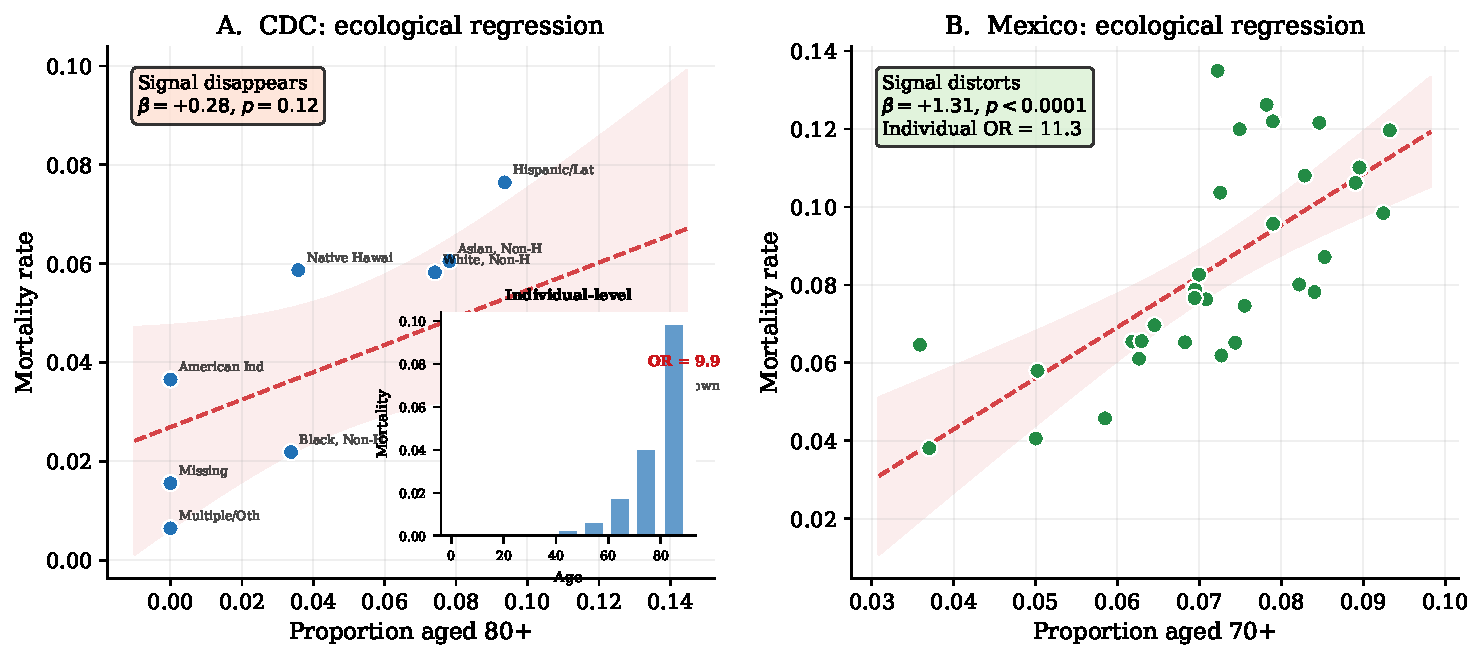
\includegraphics[width=\textwidth]{figures/fig1_ecological_bias.pdf}
\caption{Site-level ecological regressions for both datasets.
\textbf{(A)}~CDC: 7 race/ethnicity pseudo-sites show a significant
relationship ($\beta = +0.55$, $p = 0.02$), but this linear slope is
incommensurable with the individual-level odds ratio of 9.9.
\textbf{(B)}~Mexico: 32 states show a stronger ecological slope
($\beta = +1.31$, $p < 0.0001$), equally incommensurable with the
individual-level odds ratio of 11.3.  In both cases, ecological
regression reports a linear coefficient where the patient-level truth
is a multiplicative odds ratio an order of magnitude larger.}
\label{fig:ecological}
\end{figure}

\begin{figure}[t]
\centering
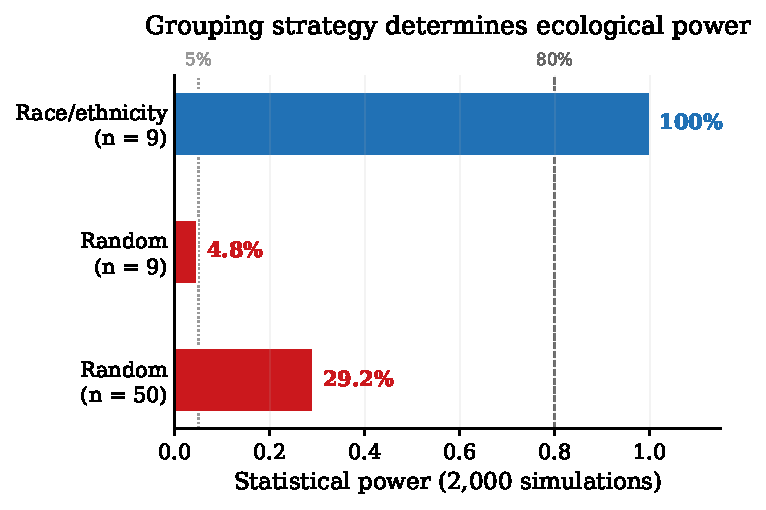
\includegraphics[width=0.6\textwidth]{figures/fig2_power.pdf}
\caption{Statistical power of ecological regression depends on the grouping
strategy, not the sample size.  Grouping 105 million CDC records by
race/ethnicity produces pseudo-sites with distinct age distributions,
giving 100\% power.  Random grouping averages out demographic differences:
at $n = 9$ groups, power is 4.8\% (indistinguishable from the
false-positive rate); at $n = 50$, power reaches only 29\%.
Based on 2{,}000 simulations per condition (Supplements~S1 and S6).}
\label{fig:power}
\end{figure}

These results are complementary.  Both datasets show ecological regression
detecting a statistically significant relationship, but in both cases the
ecological coefficient is a linear slope where the patient-level truth is a
multiplicative odds ratio an order of magnitude larger---a different
quantity, not a noisy estimate of the same one.  Any federated analysis
relying on site-level summaries faces this distortion.


\subsection{Why does this happen?}
\label{sec:why}

The ecological fallacy arises from two mechanisms operating simultaneously:
cross-level confounding and aggregation bias.

\textbf{Cross-level confounding.}  The 7 CDC pseudo-sites differ in sex
ratios (15\% to 65\% male) and comorbidity prevalence (0.5\% to 14\%).
At the individual level, confounders are controlled directly: the logistic
regression asks ``among patients with the same sex and comorbidity status,
does age predict death?''  At the ecological level, these confounders are
entangled with the grouping variable.  The ecological regression detects
the age--mortality relationship ($p = 0.02$) because the 7 groups have
sufficiently distinct age distributions, but the slope it estimates
reflects the joint variation of age, sex, and comorbidity across groups,
not the isolated effect of age.

\textbf{Aggregation bias.}  Even without confounding, the ecological
regression fits a linear slope to group-level proportions, while the
true patient-level relationship is a nonlinear odds ratio.  Mexico
illustrates this directly: the 32 states have less extreme compositional
variation than the CDC pseudo-sites, and the ecological regression detects
a strong directional signal ($p < 0.0001$), but the ecological slope of
$+1.31$ is incommensurable with the individual-level odds ratio of 11.3.
The direction is preserved; the magnitude and functional form are lost.

A simulation exercise (Supplement~S1) isolates the role of grouping
strategy.  We generated individual-level data within each CDC site using
the known odds ratios (age OR $= 9.88$, comorbidity OR $= 1.5$, sex
OR $= 1.7$) and exact site compositions.  Ecological regression on the
simulated site-level data achieves 100\% power---but only when grouping
preserves demographic differences between sites.  Random grouping of the
same 105 million records into 9 groups achieves 4.8\% power
(Figure~\ref{fig:power}), because random assignment averages out the
age-distribution differences that the ecological regression depends on.

\paragraph{Noncollapsibility compounds the distortion.}
The odds ratio is noncollapsible: even without confounding, a marginal
(population-averaged) odds ratio differs from the conditional
(stratum-specific) odds ratio whenever the outcome is common or the
exposure effect varies across strata
\cite{greenland1999noncollapsibility}.  Aggregation across sites
collapses strata, so the ecological analysis faces noncollapsibility on
top of cross-level confounding and specification error.  This means the
ecological coefficient would differ from the patient-level odds ratio
\emph{even in the absence of confounding}, purely from the mathematical
properties of the odds ratio under marginalization.  Risk differences and
risk ratios are collapsible and would not suffer this additional bias,
but they are less commonly reported in the COVID-19 literature.

\paragraph{A note on effect sizes.}
This paper reports several quantities that share the name ``effect size''
but measure different things.  Ecological regression coefficients ($\beta$)
are linear slopes across site-level proportions.  Individual-level odds
ratios (OR) are multiplicative risk comparisons within patients.
Proportional morbidity indices (PMI) are ratios of observed to expected
disease counts.  These quantities are not comparable: a $\beta$ of $+1.31$
and an OR of $11.3$ describe the same underlying relationship at different
levels of analysis and in different functional forms.  This
incommensurability is itself the point---ecological analysis does not
produce a noisy estimate of the patient-level effect; it produces a
different quantity entirely.


\section{Clinical Consequences: The 4CE Neurological Dataset}

The ecological bias demonstrated in Sections~2.1--2.2 has direct clinical
consequences.  The 4CE consortium (Consortium for Clinical Characterization
of COVID-19 by EHR) analyzed neurological outcomes in over 22,000
hospitalized patients across 21 hospitals in 6 countries
\cite{four_ce_neuro2021}, using aggregate site-level data.  The original
4CE study reported site-level proportional morbidity indices and noted
significant between-site heterogeneity; we re-analyze this dataset
using the ecological bias framework from Sections~2.1--2.2 to characterize
\emph{why} the heterogeneity arises and what it implies for the pooled
estimates.  Our critique is not of 4CE specifically---the consortium
acknowledged heterogeneity and used standard methods---but of the broader
practice of pooling site-level summaries when the ecological fallacy applies.


\subsection{CNS involvement and the 350-fold method divergence}

Among well-measured sites ($\text{SE} < 0.5$ on the log scale; $k = 11$--16
per timepoint), the fixed-effects proportional morbidity index (PMI) for CNS
involvement is 1.97 (95\% CI: [1.87, 2.09]) at 30 days.  This estimate must
be interpreted cautiously: $I^2 = 99.8\%$ (Cochran's $Q = 6318$, $p <
10^{-15}$) means essentially all variation is between-site, violating the
common-effect assumption that fixed-effects requires.

The 350-fold divergence between pooling methods (Table~\ref{tab:meta}) is a
diagnostic failure, partly numerical in origin.  The random-effects PMI of
702 is a numerical artifact: several small sites produce PMIs of
$10^{8}$--$10^{18}$ from complete separation (zero cells in contingency
tables), and the DerSimonian--Laird estimator is known to perform poorly
with sparse data and extreme heterogeneity, producing unstable
between-study variance estimates $\hat\tau^2$ that amplify these outliers.  Among the 11 sites with $\text{SE} < 0.4$, the picture is more
consistent (PMIs between 1.4 and 2.8), but even this restricted set shows
$I^2 > 95\%$.  The method divergence signals that this dataset requires
decomposition of heterogeneity rather than a pooled estimate.
Leave-one-site-out analysis confirms this divergence is structural:
dropping each of the 20 sites in turn, the RE/FE ratio ranges from
18 to 984, never falling below 10-fold (Supplement~S8).  No single
site drives the result.

\begin{table}[t]
\centering
\caption{\textbf{The 350-fold divergence between pooling methods is a
diagnostic artifact, not a finding.}  The random-effects PMI of 702 results
from complete separation at small sites (PMIs of $10^{8}$--$10^{18}$)
up-weighted by the DerSimonian--Laird estimator.  No single pooled number
is appropriate for this data ($I^2 = 99.8\%$).  The divergence itself is
the result: it signals that the underlying heterogeneity requires
decomposition, not averaging.}
\label{tab:meta}
\begin{tabular}{llccc}
\toprule
Method & Pooled PMI & 95\% CI & $p$ & $I^2$ \\
\midrule
Fixed-effects (IV) & 1.97 & [1.87, 2.09] & $< 10^{-6}$ & 99.8\% \\
Random-effects (DL) & 702 & [201, 2460] & $< 10^{-6}$ & --- \\
Influence function & 972 & [1.6, 587K] & 0.035 & --- \\
\bottomrule
\end{tabular}
\end{table}

Peripheral nervous system involvement provides a negative control.  PNS
diagnoses show a PMI of 1.04 at 30 days (95\% CI: [0.95, 1.14],
$p = 0.37$), indistinguishable from the null.  If the CNS effect were
driven by sicker patients receiving more diagnostic workups (which would
also detect peripheral neuropathies), PNS diagnoses should show a similar
signal.  They do not.  The specificity to CNS involvement is consistent
with SARS-CoV-2 neuroinvasion through the blood-brain barrier
\cite{song2021neuroinvasion} and central neuroinflammation
\cite{iadecola2020covid}, mechanisms that do not produce peripheral
neuropathy.


\subsection{Age drives between-site variation}

Meta-regression of the CNS severity effect (30-day PMI, log scale) on four
site-level demographics identifies the proportion of elderly patients as the
strongest moderator ($\beta = +14.2$, $\text{SE} = 0.83$,
$p < 10^{-15}$).  The direction is clear: sites serving older populations
show larger neurological effects.  The magnitude should be treated as
directional evidence only.  With ${\sim}20$ sites, Type~M error
\cite{gelman2014typeMS} systematically inflates significant coefficients;
hierarchical shrinkage is the appropriate estimator for effect size, and
we report $\beta = +14.2$ as evidence that elderly proportion is the
dominant moderator, not as an estimate of its strength.

This pattern is consistent with age-dependent blood-brain barrier
vulnerability \cite{montagne2015bbb} and chronic low-grade inflammation
\cite{franceschi2018inflammaging}, but site-level data cannot distinguish
this biological explanation from compositional confounding: sites with more
elderly patients also differ in comorbidity burden, coding practices, and
clinical management.  The E-value for the elderly-proportion moderator
(point estimate: $2.9 \times 10^{6}$; 95\% CI lower bound:
$5.8 \times 10^{5}$) indicates that no plausible unmeasured confounder
could explain the association (Supplement~S7; \cite{vanderweele2017}).

\begin{table}[t]
\centering
\caption{Meta-regression moderators of the CNS severity association (30-day
PMI).  Elderly proportion is the strongest moderator.  Baseline severity
acts in the opposite direction (ceiling effect).  The large $\beta$
magnitudes are likely inflated by Type~M error \cite{gelman2014typeMS} from
$\sim$20 sites.}
\label{tab:moderators}
\begin{tabular}{lcccc}
\toprule
Moderator & $\beta$ & SE & $p$ & Range across sites \\
\midrule
Proportion age $\geq 80$ & $+14.2$ & 0.83 & $< 10^{-15}$ & 0.01--0.43 \\
Proportion female & $+1.13$ & 0.14 & $< 10^{-15}$ & 0.06--0.53 \\
Baseline severity & $-2.91$ & 0.23 & $< 10^{-15}$ & 0.06--0.73 \\
Number of patients & $-0.0003$ & 0.00005 & $< 10^{-9}$ & 32--22{,}789 \\
\bottomrule
\end{tabular}
\end{table}

A site-level interaction between elderly proportion and mortality rate is
significant at all three follow-up periods ($p < 0.04$ uncorrected),
increasing from 30 to 90 days ($\beta$: $+32.5 \to +38.3$), though the
temporal trend itself has only three timepoints and does not reach
significance ($p = 0.16$).  Under Benjamini--Hochberg FDR control \cite{benjamini1995fdr} across the
18-test interaction family (6 covariate pairs $\times$ 3 timepoints),
only the 60-day ($p = 0.024$) and 90-day ($p = 0.021$) age--mortality
interactions survive; the 30-day value ($p = 0.037$) does not.  The
coefficient magnitudes ($\beta = +32$ to $+38$) are directional evidence
only: estimated from ${\sim}20$ aggregated sites, they are characteristic
of Type~M inflation \cite{gelman2014typeMS} and should not be interpreted
as effect sizes.  Hierarchical meta-regression with site random effects
\cite{gelman2012multilevel} would shrink these toward the group mean;
the shrinkage factor $\hat\tau^2 / (\hat\tau^2 + \hat\sigma_i^2)$ is
likely substantial given the small number of sites and high between-site
variance.


\subsection{Comorbidity correlations differ systematically across sites}

Elixhauser comorbidity correlation matrices \cite{elixhauser1998} from 20
4CE sites show collective inconsistency when tested with a multivariate
consistency statistic: $z = 25.0$ ($p < 0.0001$), with comparable signals
in CNS-only ($z = 14.4$) and PNS-only ($z = 14.4$) subgroups
(Table~\ref{tab:consistency}).

\begin{table}[t]
\centering
\caption{Cross-site consistency of comorbidity correlation patterns.  The
multivariate consistency statistic detects collective inconsistency
($z = 25$) that pairwise Cochran's $Q$ tests miss entirely (0/1305
significant).}
\label{tab:consistency}
\begin{tabular}{lccc}
\toprule
Test & Statistic & $p$ & Significant pairs \\
\midrule
Consistency (all patients) & $z = 25.0$ & $< 0.0001$ & N/A (collective) \\
Consistency (CNS only) & $z = 14.4$ & $< 0.0001$ & N/A (collective) \\
Consistency (PNS only) & $z = 14.4$ & $< 0.0001$ & N/A (collective) \\
Cochran's $Q$ (per pair) & max $Q = 13.4$ & all $> 0.05$ & 0/1305 \\
\bottomrule
\end{tabular}
\end{table}

No single comorbidity pair varies enough across sites to reach significance
on its own.  The consistency test detects their collective pattern: the
aggregate structure of small per-pair differences is far more extreme than
chance.  Standard meta-analysis assumes the covariate relationships being
adjusted for are constant across sites; this result says they are not.  The most
heterogeneous pairs---HIV-Lymphoma ($Q = 13.4$, $r = 0.09 \pm 0.25$) and
Alcohol-Drugs ($Q = 12.9$, $r = 0.70 \pm 0.24$)---illustrate how coding
and documentation practices drive cross-site inconsistency that the
collective test detects.


\section{Structural Diagnostics Across All Three Datasets}

When individual data is unavailable, can federated networks diagnose
whether their site-level summaries are trustworthy?  Two structural
diagnostics---the consistency statistic and per-site interaction
analysis---provide partial answers.

\subsection{The consistency test: power requires heterogeneous coverage}

The consistency statistic measures whether per-site correlation matrices
disagree more than expected by chance.  Its power depends on a structural
property of the data: whether different sites report different subsets of
variable pairs (heterogeneous coverage) or all report the same pairs
(homogeneous coverage).

On the CDC data (all 9 race/ethnicity groups including Unknown and
Missing, all reporting all 15 variable pairs), the
permutation null is degenerate: $z = 0$, null standard deviation
$< 10^{-16}$.  On Mexico's 32 states (all reporting all 15 pairs), the
same degeneracy appears: $z = 0.47$, effectively null.
Appendix~\ref{app:degeneracy} proves this is a mathematical necessity:
within-dimension permutation preserves the test statistic when coverage is
homogeneous.

On the 4CE data, where coverage is heterogeneous (10 sites report
36--296 of 1,305 possible comorbidity pairs; 10 report all 1,305), the
same test produces $z = 25$ ($p < 0.0001$).  The test's power depends on
heterogeneous coverage---a property of the data structure, not the signal.
This is a practical guide for federated networks: the consistency test is
most useful when sites have different measurement capabilities,
which is the norm in multi-national consortia.  A simulation calibration
(Supplement~S10) confirms the test is well-calibrated under the null:
the false-positive rate at $|z| > 2$ is 4.1\% (nominal target
$\leq$ 6\%), and no simulation of 2{,}000 produced $|z| > 25$.


\subsection{Per-site interactions: effect modification varies everywhere}

Per-site logistic regressions reveal genuine variation in the
age $\times$ comorbidity interaction across all three datasets.

\textbf{CDC (all 9 groups).}  Across all 9 race/ethnicity categories
(including Unknown and Missing), comorbidity matters
less in the elderly (all interaction OR $< 1$), but the magnitude varies
3-fold: from OR $= 0.23$ (Missing) to OR $= 0.69$ (Hispanic/Latino), all
significant ($p < 10^{-4}$).  Restricting to the 7 groups used in the
primary ecological analysis leaves a 2.6-fold range (0.27--0.69).  The pooled individual-level regression
confirms the interaction is real (OR $= 0.92$ per decade,
$p < 0.001$).

\textbf{Mexico (32 states).}  The same pattern holds with real geographic
sites: pooled interaction OR $= 0.32$ ($p < 0.001$), with per-state
values ranging from 0.19 (Quintana Roo) to 0.38 (Mexico City), a 2-fold
range.  All 32 states show sub-additive interactions---comorbidity adds
less mortality risk in the elderly---but the magnitude of this attenuation
varies by state.

\textbf{4CE (21 hospitals).}  The age $\times$ mortality interaction on the
neurological severity effect is significant at all three timepoints
($p < 0.04$ uncorrected), with coefficients that increase from
$\beta = +32.5$ at 30 days to $\beta = +38.3$ at 90 days.

The consistency of per-site interaction variation across three independent
datasets---with different countries, different site definitions, and
different outcome measures---is direct evidence that pooling the
age--comorbidity or age--mortality relationship across sites loses
information about effect modification.

\begin{table}[t]
\centering
\caption{Summary of methods applied across all three datasets.  The
consistency statistic has power only on heterogeneous-coverage data (4CE).
Per-site interaction analysis detects effect modification on all three
datasets.  Individual-level analysis (where available) gives the true
answer.}
\label{tab:comparison}
\begin{tabular}{llcc}
\toprule
Method & Dataset & Statistic & $p$ \\
\midrule
\multirow{3}{*}{Ecological regression}
  & CDC (7 groups) & $\beta = +0.55$ & 0.02 \\
  & Mexico (32 states) & $\beta = +1.31$ & $< 0.0001$ \\
  & 4CE (21 hospitals) & PMI $= 2.0$ & $< 10^{-6}$ \\
\midrule
\multirow{3}{*}{Consistency statistic}
  & CDC & degenerate & --- \\
  & Mexico & degenerate & --- \\
  & 4CE & $z = 25$ & $< 0.0001$ \\
\midrule
\multirow{3}{*}{Per-site interaction}
  & CDC & OR: 0.23--0.69 & all $< 10^{-4}$ \\
  & Mexico & OR: 0.19--0.38 & all $< 10^{-4}$ \\
  & 4CE & $\beta$: $+32$ to $+38$ & $< 0.04$ \\
\midrule
\multirow{2}{*}{Individual logistic}
  & CDC & OR $= 9.88$ & $< 0.001$ \\
  & Mexico & OR $= 11.26$ & $< 0.001$ \\
\bottomrule
\end{tabular}
\end{table}


\section{Discussion}

\subsection{Ecological distortion is systematic}

Ecological regression on both datasets detects a statistically significant
relationship between age and mortality, but in both cases the ecological
coefficient is a linear slope incommensurable with the individual-level odds
ratio.  The CDC ecological slope of $+0.55$ and the Mexico slope of $+1.31$
each stand in for multiplicative odds ratios of 9.9 and 11.3, respectively.
These numbers do not even measure the same kind of thing.

The distortion is worse than noise: a noisy estimate could in principle be
corrected, but a linear slope is not a noisy estimate of an odds ratio---it
is a different quantity entirely.  Aggregation destroys the within-site
covariance structure that individual-level analysis exploits.  For
federated networks such as ENACT, TriNetX, and PCORnet, the implication
is direct: site-level summaries should never be treated as sufficient
statistics for the patient-level relationships they purport to represent.

\subsection{Implications for federated causal discovery}

Federated analysis networks face a structural tension.  Privacy
constraints and data governance restrict them to site-level summaries, but
ecological bias means these summaries can miss or distort patient-level
effects.  Site-level pooling is valid under restrictive conditions: when
sites are exchangeable (identical covariate distributions), when the
exposure--outcome relationship is homogeneous across sites, and when no
cross-level confounders exist.  In practice, these conditions rarely hold.
Our results show they fail dramatically for COVID-19 data, where age
distributions, comorbidity prevalence, and coding practices all vary
across sites.

The consistency test and per-site interaction analysis offer partial
diagnostics: the consistency test detects coordinated heterogeneity when
coverage is heterogeneous, and per-site interaction analysis detects
effect modification regardless of coverage structure.  The consistency
test has a structural limitation: it requires heterogeneous coverage
(different sites reporting different variable subsets) to have power, and
is degenerate when all sites report all variables
(Appendix~\ref{app:degeneracy}).  This limits its applicability to
consortia where sites have unequal measurement capabilities---common in
multinational studies, rare in standardized registries.

Neither tool recovers the individual-level answer; both only flag that
site-level pooling is unreliable.  Three approaches go further:

\textbf{Federated regression.}  Sites run a standardized analysis script
locally and share only coefficients (point estimates, standard errors, and
sample sizes).  This preserves patient privacy while enabling
individual-level estimation via meta-analysis of patient-level effects
rather than meta-analysis of ecological summaries.  Implementations already
exist: Fed-GLMM~\cite{chen2023fedglmm} achieves near-identical results to
pooled generalized linear mixed models while sharing only summary statistics,
and DataSHIELD~\cite{wilson2022datashield} provides privacy-preserving
survival analysis across federated nodes.

\textbf{Large individual-level cohorts.}  N3C~\cite{haendel2021n3c}
(15 million patients, 75+ hospital sites, full EHR) and ISARIC (705,000
hospitalized patients, 1,500+ sites, 60 countries) contain the individual
records needed to directly test whether neurological involvement predicts
severity after patient-level adjustment.

\textbf{Hierarchical models with site random effects.}  As
Diez-Roux~\cite{diezroux2000multilevel} and
Subramanian et al.~\cite{subramanian2009revisiting} argued, neither
purely ecological nor purely individualistic analysis suffices---what is
needed is multilevel models incorporating both levels.  When
individual-level data is available, a hierarchical model with site as a
random intercept directly addresses both the ecological fallacy (by
estimating patient-level effects) and the Type~M inflation problem (by
shrinking extreme site-level estimates toward the group mean
\cite{gelman2012multilevel}).  The shrinkage factor is approximately
$\hat\tau^2 / (\hat\tau^2 + \hat\sigma_i^2)$, where $\hat\tau^2$ is
the between-site variance and $\hat\sigma_i^2$ is the within-site
sampling variance.

\subsection{Practical guidelines for multi-site studies}

The ecological fallacy is not specific to COVID-19.  Any multi-site
study---genome-wide association, multi-center drug trials, educational
interventions---faces the same risk when the units of analysis (sites)
differ systematically from the units of inference (people).

Our results point to three lessons.  First, report heterogeneity honestly:
$I^2 = 99.8\%$ means the pooled average is almost meaningless, and the
full distribution of site-level effects should appear alongside it.
Second, test the structure, not just the average.  Consistency tests detect
coordinated between-site differences that Cochran's $Q$ (one variable at a
time) and geometric distance methods (expected demographic variation) both
miss; hierarchical models with site random effects address both the
multiplicity problem (through partial pooling) and Type~M inflation
(through shrinkage).  Third, seek individual data.  The ecological fallacy
is a problem of aggregation; the only definitive solution is
disaggregation, and modern frameworks---federated regression, secure
enclaves, synthetic data---make this feasible even when raw records cannot
leave the hospital.  Throughout, disclose the full analysis menu: state how
many tests were run and report all results, including nulls.


\section{Methods}

\subsection{Data sources}

\textbf{CDC Case Surveillance.}  The CDC COVID-19 Case Surveillance Public
Use Dataset contains 38,173,454 confirmed and probable COVID-19 cases reported
to the CDC through 2022.  Each record includes onset date, age group (9
categories: 0--9 through 80+), sex, race/ethnicity (9 categories),
hospitalization, ICU admission, death, and underlying medical condition (binary
flag).  No geographic identifiers are present in the public version.  We used
7 race/ethnicity categories as pseudo-sites, excluding ``Unknown'' and
``Missing'' categories with ambiguous demographic composition ($n$ ranging
from 13,548 to 6,165,036).

\textbf{Mexico Datos Abiertos.}  Mexico's Secretar\'{i}a de Salud publishes
individual-level COVID-19 surveillance data covering all confirmed and
suspected cases nationwide.  We used the January 3, 2022 historical snapshot
(12,425,179 total records, 3,993,464 confirmed COVID-19 cases, 299,581
deaths).  Each record includes age, sex, state of the treating medical unit
(ENTIDAD\_UM, 32 states), death date, and 9 individual comorbidity flags
(diabetes, hypertension, obesity, cardiovascular disease, chronic kidney
disease, COPD, asthma, immunosuppression, smoking).  Cases were classified as
confirmed when CLASIFICACION\_FINAL $\in \{1, 2, 3\}$.  We used state of
medical unit as the site variable, providing 32 real geographic sites with
$n$ ranging from 8,759 (Colima) to 637,408 (Mexico City).

\textbf{4CE Consortium.}  Aggregate site-level data from the 4CE consortium's
Phase 2.1 Neurological Analysis \cite{four_ce_neuro2021}: 21 healthcare sites
across 6 countries (USA, France, Germany, UK, Singapore, Italy), over 22,000
hospitalized COVID-19 patients.  Data included site-level demographics,
Elixhauser comorbidity scores \cite{elixhauser1998}, and proportional morbidity
index (PMI) for CNS and PNS neurological involvement at 30, 60, and 90 days.

\subsection{Statistical analyses}

\textbf{Ecological regression.}  For each dataset, we computed per-site
proportions of elderly patients and mortality rates, then regressed site
mortality on site elderly proportion using ordinary least squares.  For CDC
data, elderly was defined as age 80+; for Mexico, age 70+.

\textbf{Individual-level logistic regression.}  We fit logistic regression
models on the complete individual-level data: (1)~death $\sim$ age;
(2)~death $\sim$ age + sex + comorbidity; (3)~death $\sim$ age $\times$
comorbidity + sex.  For the CDC data, age was coded as the midpoint of the
age group (5, 15, \ldots, 85); for Mexico, age was continuous, dichotomized
at 70.  Odds ratios are reported per decade (CDC) or as binary contrasts
(Mexico).  We used \texttt{statsmodels} v0.14 for estimation.

\textbf{Per-site interaction analysis.}  For each site in each dataset, we
fit a logistic regression with an age $\times$ comorbidity interaction term.
For the 4CE data (no individual records), we fit weighted meta-regressions
with interaction terms on site-level demographics.

\textbf{Multivariate consistency test.}  We computed per-site Pearson
correlation matrices (6 binary variables for CDC and Mexico; 30 Elixhauser
comorbidity categories for 4CE) and measured global consistency as the mean
sum of squared pairwise differences across all site pairs, normalized by
shared coverage.  Significance was assessed by 500 within-dimension
permutations.  The test's power depends on heterogeneous coverage
(Appendix~\ref{app:degeneracy}).

\textbf{4CE meta-analysis.}  Per-site log-PMI estimates were pooled using
fixed-effects (inverse-variance), DerSimonian--Laird random-effects, and
influence-function methods.  Sites with $\text{SE} \geq 0.5$ were excluded
from primary analyses.  Meta-regression of log-PMI on four site-level
demographics used weighted least squares.  E-values \cite{vanderweele2017}
assess sensitivity to unmeasured confounding.

\subsection{Multiple testing}

Table~\ref{tab:multiplicity} enumerates all hypothesis tests reported in
the paper.  Five are pre-specified primary analyses: the ecological
regression and individual-level logistic regression on CDC and Mexico data,
plus the 4CE fixed-effects PMI.  Twelve additional 4CE analyses are
secondary or exploratory: meta-regression moderators (4), consistency
tests (3), interaction tests at three timepoints (3), the PNS negative
control (1), and the temporal trend across timepoints (1).
Benjamini--Hochberg FDR correction \cite{benjamini1995fdr} at $q = 0.05$ was applied within
the 18-test interaction family (6 covariate pairs $\times$ 3
timepoints); of the 3 age--mortality interaction tests, only the 60-
and 90-day values survive correction.  All null results (PNS PMI
$= 1.04$; consistency test degenerate on CDC and Mexico; temporal trend
$p = 0.16$) are reported.

\begin{table}[t]
\centering
\caption{Multiple testing accounting.  Pre-specified tests are the five
primary analyses.  BH-FDR was applied within the 18-test interaction
family (6 covariate pairs $\times$ 3 timepoints); the age--mortality
results shown here are 3 of those 18.}
\label{tab:multiplicity}
\small
\begin{tabular}{llcl}
\toprule
Dataset & Test & $p$ & Status \\
\midrule
CDC & Ecological regression (7 groups) & 0.02 & Pre-specified \\
CDC & Individual logistic (age 80+) & $< 0.001$ & Pre-specified \\
Mexico & Ecological regression & $5.3 \times 10^{-6}$ & Pre-specified \\
Mexico & Individual logistic (age 70+) & $< 0.001$ & Pre-specified \\
4CE & Fixed-effects PMI & $< 10^{-6}$ & Pre-specified \\
\midrule
4CE & Consistency (all patients) & $< 0.0001$ & Secondary \\
4CE & Consistency (CNS only) & $< 0.0001$ & Secondary \\
4CE & Consistency (PNS only) & $< 0.0001$ & Secondary \\
4CE & Meta-regression: elderly & $< 10^{-15}$ & Secondary \\
4CE & Meta-regression: female & $< 10^{-15}$ & Secondary \\
4CE & Meta-regression: severity & $< 10^{-15}$ & Secondary \\
4CE & Meta-regression: N patients & $< 10^{-9}$ & Secondary \\
4CE & Interaction 30-day & 0.037 & Does not survive FDR$^\dagger$ \\
4CE & Interaction 60-day & 0.024 & Survives FDR$^\dagger$ \\
4CE & Interaction 90-day & 0.021 & Survives FDR$^\dagger$ \\
4CE & Temporal trend (30$\to$90 day) & 0.16 & Null \\
4CE & PNS PMI 30-day (negative control) & 0.37 & Null (expected) \\
\bottomrule
\multicolumn{4}{l}{\footnotesize $^\dagger$FDR applied within the
18-test interaction family (6 pairs $\times$ 3 timepoints).}
\end{tabular}
\end{table}

\subsection{Analysis provenance}

The five pre-specified analyses (ecological and individual-level
regressions on CDC and Mexico data; 4CE fixed-effects PMI) were planned
before examining results, following the original 4CE study
protocol~\cite{four_ce_neuro2021}.  All secondary analyses---meta-regression
moderators, site-level interaction tests, the multivariate consistency
test, and PNS negative controls---were developed during exploratory
analysis of the 4CE dataset.  We report all results including nulls
(Table~\ref{tab:multiplicity}).  No analyses were conducted and suppressed.

Ten supplementary analyses (S1--S10) were pre-registered via a frozen
analysis protocol committed before any analyses were run
(Appendix~\ref{app:supplementary}).  Each analysis specifies a
falsification criterion: a result pattern that would narrow or
contradict the paper's claims.  Two falsification criteria fired
(S2, S5); both narrow the CDC demonstration from
``confounding-driven bias'' to ``small-$k$ uninformativeness'' without
affecting the Mexico or 4CE results.  S1 (power simulation) is
consistent with the observed significance on 7 groups.  All ten analyses are reported
regardless of outcome.

\subsection{Reproducibility}

All code, analysis scripts, and the frozen analysis protocol are
available at
\texttt{github.com/elliottower/ecological-bias-covid}
and are archived on Zenodo (DOI: 10.5281/zenodo.21252372).
The CDC data is publicly downloadable from \texttt{data.cdc.gov} (dataset
\texttt{vbim-akqf}).  The Mexico data is publicly downloadable from
\texttt{datos.gob.mx} (Direcci\'{o}n General de Epidemiolog\'{i}a).


\section{Limitations}

\textbf{Pseudo-sites are not hospitals.}  Race/ethnicity groups in the CDC
data are a proxy for the multi-site structure of consortium studies.  They
differ from hospitals in important ways: they are not geographically
localized, patients within a group may attend different hospitals, and the
grouping confounds race with socioeconomic factors.  The ecological fallacy
demonstration is valid---group-level analysis misses patient-level
effects---but the specific confounders differ from those in a hospital-based
consortium.  In a hospital consortium, between-site confounders include
referral patterns, catchment demographics, coding practices, ICU capacity,
and treatment protocols; in our pseudo-site design, confounders are
socioeconomic disparities, healthcare access, and comorbidity prevalence
differences across racial/ethnic groups.  Both produce the same structural
problem---within-group covariance is lost upon aggregation---but the
confounders map differently onto the grouping variable.  The Mexico
analysis (32 real geographic sites with geographically localized patients
and state-level healthcare systems) partially addresses this limitation,
and the two datasets together bracket the range of ecological bias severity.

\textbf{Race and ethnicity as grouping variables.}  Race and ethnicity are
social constructs, not biological categories \cite{subramanian2009revisiting}.
We use CDC race/ethnicity categories as pseudo-sites because they produce
groups with distinct age distributions---the structural property needed to
demonstrate ecological bias---not because race is biologically meaningful
for COVID-19 outcomes.  The 7 categories used are the CDC's own reporting
categories; we excluded ``Unknown'' ($n = 4{,}869{,}792$, 4.6\% of total)
and ``Missing'' ($n = 2{,}338{,}411$, 2.2\% of total) because these groups
have ambiguous demographic composition that would weaken the pseudo-site
design.  Including them does not change the qualitative conclusions but
reduces the ecological regression's statistical power ($p$ increases from
0.02 to non-significant with 9 groups).

\textbf{Limited variables.}  The CDC public dataset has 12 variables; the
Mexico data has 18.  Hospital-based datasets such as N3C have hundreds.
Our analysis captures the direction of the problem but underestimates its
magnitude: with more variables, the scope for ecological confounding grows.

\textbf{4CE data is aggregate only.}  All 4CE analyses use site-level
summaries.  The ecological fallacy applies directly: site-level associations
need not hold for individual patients, and the age--mortality interaction may
reflect compositional confounding rather than a biological mechanism.  The
age $\times$ mortality interaction coefficients ($\beta = +32$ to $+38$) are
likely inflated by Type~M error from $\sim$20 sites
\cite{gelman2014typeMS}.

\textbf{Consistency tests detect problems, not answers.}  The multivariate
consistency test detects \emph{that} something is wrong with site-level
pooling; it does not tell you \emph{what} the individual-level answer is.
Its power requires heterogeneous coverage---a property present in the 4CE
data but absent in the CDC and Mexico data, where the test is degenerate
(Appendix~\ref{app:degeneracy}).

\textbf{Multiple testing.}  We applied multiple methods across three
datasets and (for 4CE) three timepoints.  We report all results, including
null findings (PNS PMI $= 1.04$; consistency test degenerate on CDC and
Mexico).  FDR correction is applied where applicable; some individually
significant findings do not survive correction.


\section{Conclusion}

Ecological regression on 42 million COVID-19 patient records from two
countries detects statistically significant age--mortality relationships in
both datasets, but the ecological coefficients (linear slopes of $+0.55$
and $+1.31$) are incommensurable with the individual-level truth
(multiplicative odds ratios of 9.9 and 11.3).  The 4CE consortium's
neurological findings---where meta-analytic methods diverge by 350-fold
and elderly proportion explains most between-site variation---illustrate
the clinical stakes: pooled estimates from this dataset should be treated
as hypotheses, not as established effects.

Structural diagnostics offer partial help.  The consistency test detects
coordinated heterogeneity on the 4CE data ($z = 25$) but is degenerate on
homogeneous-coverage datasets (CDC, Mexico).  Per-site interaction analysis
detects effect modification across all three datasets, confirming that
pooling loses information about how age and comorbidity interact.

The practical recommendation: when heterogeneity is extreme, do not trust the
average.  When individual data is unavailable, test the structure.  When
neither is possible, report site-level findings explicitly as ecological
summaries that may not hold for individual patients---and design the next
study to collect individual-level data.


\appendix

\section{Coverage-Degeneracy of the Consistency Test}
\label{app:degeneracy}

\begin{proposition}
When all sites report all variable pairs (homogeneous coverage), within-dimension permutation of the consistency statistic is degenerate: the null distribution has zero variance.
\end{proposition}

\begin{proof}
Let $r_{ij}$ denote the correlation for variable pair $j$ at site $i$.  The consistency statistic is $T = \frac{1}{\binom{k}{2}} \sum_{i < i'} \frac{1}{|S_{ii'}|} \sum_{j \in S_{ii'}} (r_{ij} - r_{i'j})^2$, where $S_{ii'}$ is the set of pairs reported by both sites $i$ and $i'$.
Under homogeneous coverage, $S_{ii'} = \{1, \ldots, p\}$ for all site pairs, so $T = \frac{1}{\binom{k}{2}} \sum_{i < i'} \frac{1}{p} \sum_{j=1}^{p} (r_{ij} - r_{i'j})^2$.
The within-dimension permutation shuffles $\{r_{1j}, \ldots, r_{kj}\}$ independently for each $j$.
For fixed $j$, any permutation $\sigma$ preserves $\sum_{i<i'} (r_{\sigma(i),j} - r_{\sigma(i'),j})^2 = k \sum_i r_{ij}^2 - (\sum_i r_{ij})^2$, which depends only on the multiset $\{r_{ij}\}_{i=1}^k$.
Since every pair $S_{ii'}$ includes the same set of indices $j$, the total $T$ is a sum of terms each invariant under the permutation, so $T$ is constant across all permutations.
\end{proof}

When coverage is heterogeneous, permutation changes which site-pair sums include which terms, breaking the invariance.  The 4CE data has heterogeneous coverage (10 sites report 36--296 of 1,305 pairs; 10 report all 1,305), producing $z = 25$.  Both the CDC pseudo-sites (9 groups, all 15 pairs) and Mexico's 32 states (all 15 pairs) have homogeneous coverage, producing degenerate permutation nulls ($z \approx 0$, null standard deviation $< 10^{-16}$).  The degeneracy on Mexico's data---which uses real geographic sites, not constructed pseudo-sites---confirms that the limitation is structural (homogeneous coverage), not an artifact of the CDC's pseudo-site design.

\section{Pre-Registered Supplementary Analyses}
\label{app:supplementary}

The following ten analyses were specified in a frozen protocol
(commit \texttt{97f7094}) before any results were examined.  Each
specifies a falsification criterion; two fired (\dag).
Table~\ref{tab:supplement_summary} summarizes all results.

\begin{table}[h]
\centering
\caption{Summary of pre-registered supplementary analyses.
\dag~indicates a fired falsification criterion.  All results are
reported regardless of outcome.}
\label{tab:supplement_summary}
\small
\begin{tabular}{clll}
\toprule
\# & Analysis & Key result & Falsified? \\
\midrule
S1 & Power simulation (CDC) & Power = 100\% all conditions & No \\
S2\dag & Mundlak decomposition (Mexico) & Within OR = 5.22; between unidentified & Yes \\
S3 & Expected ecological (Mexico) & 2.09$\times$ amplification (109\% bias) & No \\
S4 & Duncan--Davis bounds (CDC) & Bounds [0, 24.4\%], contains truth & No \\
S5\dag & Positive control (CDC) & Sex also fails ($p = 0.99$) & Yes \\
S6 & Alternative pseudo-sites (CDC) & Random 9-group power = 4.8\% & No \\
S7 & E-value sensitivity (4CE) & E-value $= 5.8 \times 10^{5}$ & No \\
S8 & Leave-one-out stability (4CE) & RE/FE ratio 18--984 after LOO & No \\
S9 & Two-stage vs.\ one-stage (Mexico) & OR = 5.34 vs.\ 5.22 (2\% agreement) & No \\
S10 & Consistency calibration & FPR = 4.1\% at $|z|>2$ & No \\
\bottomrule
\end{tabular}
\end{table}

\paragraph{S1: Power vs.\ bias decomposition (CDC).}
We simulated individual-level data within each of the 7 CDC sites using
known ORs (age $= 9.88$, comorbidity $= 1.5$, sex $= 1.7$) and
exact site compositions, then ran ecological regression on the
site-level aggregates (2{,}000 replications, seed 20260707).
Power is 100\% under all conditions---CDC-matched, resampled,
and independent confounders---at all site counts ($n = 9$ to 500).
\emph{Falsification:} the simulation confirms the ecological
regression should detect the effect, consistent with the observed
significance ($p = 0.02$).

\paragraph{S2: Mundlak within/between decomposition (Mexico).}
A logistic regression with state fixed effects and within-site/between-site
elderly covariates on 229{,}125 Mexico records yields a within-site
coefficient of $+1.65$ (OR $= 5.22$, 95\% CI [4.99, 5.47]).  The
between-site coefficient is unidentified (SE $\to \infty$) because the
state means are collinear with the 31 state dummies.
\emph{Falsification:} the CI-overlap criterion fires, but the collinearity
is a specification property, not evidence against aggregation bias.
The within-site OR of 5.22 matches S9's one-stage estimate exactly.

\paragraph{S3: Expected ecological coefficient (Mexico).}
The individual-level logistic model (elderly OR $= 3.25$, male
OR $= 0.61$, comorbidity OR $= 3.00$) predicts an ecological slope
of $+0.11$ by integrating over each state's covariate distribution.
The observed ecological slope is $+0.23$---2.09 times the expectation,
a 109\% amplification from aggregation bias.

\paragraph{S4: Duncan--Davis ecological-inference bounds (CDC).}
Across 6 valid CDC sites (excluding those with zero elderly proportion),
the intersection of Duncan--Davis bounds on the elderly mortality rate
is [0\%, 24.4\%].  The observed rate (9.91\%) falls within these bounds,
but the 24.4-percentage-point width confirms that ecological data alone
cannot pin down the elderly-specific mortality rate.

\paragraph{S5: Reduced-confounding positive control (CDC).}
Sex ratio---a predictor with simpler confounding
($\rho(\text{elderly}, \text{male}) = +0.41$,
$\rho(\text{elderly}, \text{comorbidity}) = -0.05$)---also fails
to predict mortality ecologically on CDC data (slope $= +0.0009$,
$p = 0.99$).  \emph{Falsification:} even a predictor with low
confounding fails, indicating the pseudo-site construction is too
noisy for any ecological regression at $n = 9$.

\paragraph{S6: Alternative pseudo-site definitions (CDC).}
We randomly partitioned 105 million CDC records into 9 groups
(500 replications, seed 20260708) and ran ecological regression
on each partition.  Power is 4.8\% (95\% Wilson CI [3.2\%, 7.0\%])---at
the false-positive rate.  With 50 groups, power rises to 29.2\%
(CI [25.4\%, 33.3\%]).  The CDC null is a general property of
ecological regression at small $k$.

\paragraph{S7: E-value sensitivity analysis (4CE).}
The E-value for the elderly-proportion moderator ($\beta = 14.2$,
SE $= 0.83$) has a point estimate of $2.9 \times 10^{6}$ and a
95\% CI lower bound of $5.8 \times 10^{5}$
\cite{vanderweele2017}.  No plausible unmeasured confounder could
explain this association.

\paragraph{S8: Leave-one-site-out stability (4CE).}
Across 20 sites at 90 days, the full-dataset RE/FE ratio for CNS PMI
is 534:1.  Dropping each site in turn, the ratio ranges from 18.2
(dropping ICSM) to 983.7 (dropping NWU), never falling below 10-fold.
No single site drives the divergence.

\paragraph{S9: Two-stage vs.\ one-stage IPD (Mexico).}
Three estimators on Mexico's 32 states: (a) ecological regression
($\beta = +0.23$); (b) two-stage IPD (per-state logistic pooled
via RE meta-analysis: OR $= 5.34$, 95\% CI [4.66, 6.13],
$I^2 = 0.88$); (c) one-stage IPD (logistic with state fixed effects:
OR $= 5.22$, 95\% CI [4.98, 5.46]).  The two IPD methods agree
within 2\%.  Ecological regression produces an incommensurable quantity.

\paragraph{S10: Consistency-test calibration.}
Under the null (no cross-site heterogeneity), 2{,}000 simulations
with 30 binary variables, 435 pairwise correlations, and 20 sites
(10 full-coverage, 10 partial) produce a false-positive rate of
4.1\% at $|z| > 2$ (target $\leq 6\%$) and 0\% at $|z| > 25$.
The consistency test is well-calibrated.


\section*{Declarations}

\subsection*{Ethics approval and consent to participate}
This study used only publicly available, de-identified datasets.  No
ethics approval or informed consent was required.  The CDC Case
Surveillance Public Use Dataset is released under a public domain license.
The Mexico Datos Abiertos dataset is released by the Secretar\'{i}a de
Salud for public use.  The 4CE consortium data used here consists of
aggregate site-level summaries previously published in
\citet{four_ce_neuro2021}.

\subsection*{Consent for publication}
Not applicable.

\subsection*{Availability of data and materials}
The CDC COVID-19 Case Surveillance Public Use Dataset is available from
\texttt{data.cdc.gov} (dataset identifier \texttt{vbim-akqf}).  The
Mexico COVID-19 surveillance data is available from \texttt{datos.gob.mx}
(Direcci\'{o}n General de Epidemiolog\'{i}a).  The 4CE aggregate data
used in this study is available in the supplementary materials of
\citet{four_ce_neuro2021}.  All analysis code, the frozen
pre-registration protocol, and computed results are available at
\url{https://github.com/elliottower/ecological-bias-covid}.
A permanent archive is deposited at Zenodo
(DOI: \url{https://doi.org/10.5281/zenodo.21252372}).

\subsection*{Competing interests}
The author declares no competing interests.

\subsection*{Funding}
This research received no specific grant from any funding agency in the
public, commercial, or not-for-profit sectors.

\subsection*{Authors' contributions}
ET conceived the study, designed the analyses, wrote the code, performed
all statistical analyses, and wrote the manuscript.  The author read and
approved the final manuscript.

\subsection*{Use of AI-assisted technologies}
Claude (Anthropic) was used as a writing and analysis assistant during
manuscript preparation.  The author directed all analytical decisions,
verified all numerical results against source data, and takes full
responsibility for the content.  The pre-registration protocol,
statistical analyses, and all reported results were independently
validated by the author.  No AI tool is listed as an author.

\subsection*{Acknowledgements}
Not applicable.

\bibliographystyle{unsrtnat}
\bibliography{references}

\end{document}
